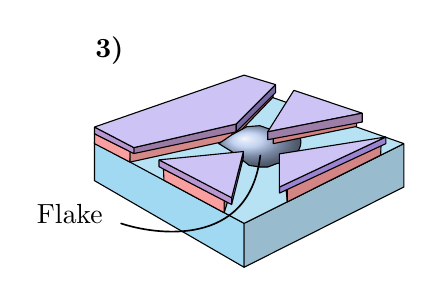
\begin{tikzpicture}

\draw[line join=bevel, fill=cyan!89!violet!40] (0,1.17) -- (0,0.68) -- (1.9,-0.42) -- (1.9,0.138) -- cycle;
\draw[line join=bevel, fill=cyan!87!purple!34!lightgray] (1.9,0.138) -- (3.93,1.15) -- (3.93,0.6) -- (1.9,-0.42) -- cycle;
\draw[fill=cyan!91!purple!31, line join=bevel, draw opacity=1, fill opacity=1] (0,1.158) -- (1.9,1.863) -- (3.93,1.15) -- (1.9,0.138) -- cycle;
\draw[line join=bevel, fill=lightgray!90!black!70!red, fill opacity=1] (1.846,1) -- (1.856,0.94) -- (1.646,0.27) -- (1.646,0.43) -- cycle;
\draw[line join=bevel, fill=pink!97!teal!84!red, fill opacity=1] (0,1.276) -- (0,1.15) -- (0.451,0.916) -- (0.453,1.05) -- cycle;
\draw[line join=bevel, fill=lightgray!95!pink!71!red, fill opacity=1] (0.453,1.05) -- (0.453,0.916) -- (1.748,1.2) -- (1.748,1.325) -- cycle;
\draw[line join=bevel, fill=gray!86!white!77!red, fill opacity=1] (2.27,1.8) -- (2.267,1.74) -- (1.748,1.2) -- (1.748,1.325) -- cycle;
\draw[fill, shade, shading=ball, ball color=blue!74!green!32] (1.742,1.05) -- (1.579,1.15) -- (1.742,1.261) -- (1.934,1.365) -- (2.1,1.378) -- (2.362,1.286) -- (2.617,1.216) .. controls (2.628,1.156) and (2.617,1.1) .. (2.582,1.05) -- (2.633,0.874) -- (2.324,0.9) -- (2.2,0.853) -- (2.1,0.853) -- (1.965,0.874) -- cycle;
\draw[line join=bevel, fill=cyan!51!magenta!81!orange, fill opacity=1] (0.5,1.1) -- (0.5,1.024) -- (1.8,1.3) -- (1.8,1.4) -- cycle;
\draw[line join=bevel, fill=purple!80!magenta!59!cyan, fill opacity=1] (2.3,1.9) -- (2.3,1.8) -- (1.8,1.3) -- (1.8,1.4) -- cycle;
\draw[line join=bevel, fill=white!87!magenta!72!blue, fill opacity=1] (0,1.361) -- (0,1.276) -- (0.5,1.024) -- (0.5,1.1) -- cycle;
\draw[line join=bevel, fill=pink!97!teal!84!red, fill opacity=1] (0.876,0.829) -- (0.882,0.685) -- (1.646,0.273) -- (1.646,0.43) -- cycle;
\draw[line join=bevel, fill=white!87!magenta!72!blue, fill opacity=1] (0.82,0.944) -- (0.82,0.857) -- (1.742,0.376) -- (1.742,0.467) -- cycle;
\draw[line join=bevel, fill=blue!70!orange!56, fill opacity=1] (1.891,1.05) -- (1.891,0.975) -- (1.742,0.376) -- (1.742,0.477) -- cycle;
\draw[line join=bevel, fill=white!77!blue!85!pink] (0.82,0.944) -- (1.891,1.05) -- (1.742,0.463) -- cycle;
\draw[fill=white!77!blue!85!pink, line join=bevel] (0,1.361) -- (0.5,1.1) -- (1.8,1.4) -- (2.3,1.9) -- (1.9,2.02) -- cycle;
\draw[fill=lightgray!99!gray!69!red, line join=bevel] (2.448,0.644) -- (2.448,0.41) -- (3.634,1.005) -- (3.64,1.15) -- cycle;
\draw[fill=pink!97!teal!84!red, line join=bevel] (2.448,0.42) -- (2.426,0.636) -- (2.448,0.706) -- (2.448,0.6) -- cycle;
\draw[fill=white!77!blue!85!pink, line join=bevel] (2.532,1.827) -- (2.2,1.3) -- (3.4,1.537) -- cycle;
\draw[fill=red!96!teal!34!lightgray, line join=bevel] (2.27,1.245) -- (2.27,1.15) -- (3.327,1.368) -- (3.332,1.45) -- cycle;
\draw[fill=cyan!56!brown!63!magenta, line join=bevel] (2.2,1.3) -- (2.2,1.2) -- (3.4,1.424) -- (3.4,1.537) -- cycle;
\draw[fill=blue!68!orange!58, line join=bevel] (3.7,1.235) -- (3.7,1.15) -- (2.35,0.522) -- (2.349,0.6) -- cycle;
\draw[fill=white!77!blue!85!pink, line join=bevel] (2.349,0.599) -- (2.349,1.02) -- (3.7,1.235) -- cycle;



  \node at (-0.314,0.26) {Flake};
  \draw[semithick, line cap=round] (2.106,1) .. controls (1.965,-0.2) and (0.74,0) .. (0.337,0.137);

  \node at (0.19,2.33) {\textbf{3)}};
\end{tikzpicture}